\chapter{Writing a Lab Report}

\section{Objective}

To learn how to write a lab report. 

\section{Introduction}

Writing how to report an experiment you have done is one of the most important skills you will learn in the lab. The lab report starts from your log book, in which you make notes on the various stages of the experiment as you do it: (i) planning and designing the experiment, (ii) making observations, (iii) analysing data and doing relevant calculations, including error analysis (iv) interpreting your results in light of the theoretical background. What you write in your log book is to the lab report what the initial sketches of an artist are to the final work of art that she produces.

You will perhaps also want to remember that your lab report will be graded. Here are some things that you should keep in mind; they are what your instructor and teachings fellows will notice.

Make your lab report \textbf{clear} and \textbf{easy to follow}. A common mistake students make is to write extremely long and elaborate reports that convey very little. We are not looking for pages and pages of writing; in fact, from experience, we have seen that the best reports are usually \textbf{short}. It is your job to decide what is relevant and what isn't. (This is good training for the future.) What you decide to include should be arranged logically and have a certain flow. 

\begin{imp}
Your lab report may be written by hand, on Microsoft Word, or using \LaTeX. Of these options, we suggest you begin using \LaTeX\, as soon as possible: it makes your work look professional, and learning to use it is good practice.
\end{imp}

\textbf{Data does not lie.} Contrary to popular opinion, grades are not assigned on how close the value obtained agrees with the ``correct'' one. If you are supposed to verify a law of nature, and you end up disproving it, that's fine, provided that you say that you have disproved it. If however you could not verify it but say that you did, we can only assume that you didn't understand the experiment. If your results are completely different from established values, then you have probably measured or calculated something incorrectly. 

\begin{imp}
The lab report should contain \textbf{all} the information required for someone else to reproduce your experiment \textbf{and} its results.

\textbf{A non-standard answer with a clear path as to how you got there is worth significantly more than a standard answer that appears unjustified or out of nowhere. }
\end{imp}

The handouts contain questions about the experiment are scattered around the manual. Make sure you try to answer them as you write your report; these questions are included at critical points to check your comprehension, and the answers often provide ideas of what to include in a good report. 

\begin{imp}
Spend some time thinking about the format of your lab report. We don't expect something publishable in \textit{Physical Review Letters}, but on the other hand, we don't expect four pages of stream-of-consciousness writing either.
\end{imp}

\section{Essential Elements of a Report}

As stated above the the lab report should contain all the information needed for someone else to redo the experiment. This means that the following need to be written:

\begin{enumerate}
    \item A brief introduction to the experiment, including the aim, the approach to be followed, and a statement of the theoretical background, if needed. (In the introductory lab, enough theoretical background is generally provided, but that may not be true in later labs; in that case you may want to include some of the theory needed to understand the experiment.)
    \item The equipment used, with details. The details of the instruments don't need to be provided at the beginning but should be provided in the section where they are actually used. For example, if you are using Vernier calipers to measure the diameter of a set of balls, you need to specify the least count of the main scale and of the Vernier scale just before the table with the data on the diameters. 
    \item The procedure followed. This section should be very clear, and actually state the procedure \textit{you} followed, not what some book says you ought to have followed. 
    \item The data, clearly tabulated. As stated above, each table should be preceded by the details of the instrument used to collect the data.
    \item Error analysis, if needed.  
    \item Graphs, where needed.
    \item The result, clearly stated. 
    \item A discussion of the difficulties encountered, and any ideas that may have occurred to you for improvement of the experiment, or other related experiments that could be done.
    
\end{enumerate}

\subsubsection{Tables, Figures, and Graphs}

Tables, Figures, and Graphs (which we will come to in the next session) have a required standard of presentation, usually much higher than those you might put in your log book. If possible, have any tables and figures at the top and/or bottom of a page, and do not wrap text around figures or tables.

\begin{imp}
In general, you may use any software for data analysis. Beginners will usually prefer to use Microsoft Excel or Google Sheets. However, as you progress, it is \textbf{very strongly} advised that you use this lab to learn how to do very elementary plotting and data analysis using Python and Jupyter Notebook. We will come to this in the next session.
\end{imp}

\paragraph{Figures:} 
\begin{enumerate}
    \item The figures you will include in your lab report will usually be descriptions of the apparatus or schematic diagrams. 
    \item In general, they should be well marked and labelled and you should be able to refer to them through the report to better explain what you've done. 
    \item All figures should have a label (such as ``Figure 1:'' or ``Fig.1:'') at the start of a caption explaining what they describe. 
    \item Captions should be short and sufficiently informative so that anyone with some knowledge of the experiment will understand what it represents without having to refer to your report.
\end{enumerate}

\paragraph{Graphs:}
\begin{enumerate}
    \item Your graphs should be easy to read and clearly show all key features.
    \item Graphs are figures, and should therefore have a figure number at the start of their caption (``Fig.1:'', not ``Graph 1:'').
    \item Consider whether various results can be combined into a single graph.
    \item Here are some things your graph \textbf{must} have:
    
    \begin{enumerate}
        \item Labelled axes with units,
        \item Error bars, indicating the uncertainty with which you know the location of the point,
        \item A white background,
        \item Sensible maximum and minimum values so that most of the space is filled by the graph.
    \end{enumerate}
    
    \item Your graph \textbf{does not} need to have:
    
    \begin{enumerate}
        \item A title: all the information about the graph should be in the caption,
        \item Grid-marks or a border,
        \item Legends (unless the graph cannot be understood without one): this information would preferably also go into the caption.
    \end{enumerate}

\end{enumerate}


\paragraph{Tables:}

\begin{enumerate}
    \item Like figures, tables should be labelled and have a caption. However, they are \textbf{not} figures, but should instead be labelled ``Table 1:'', etc.
    \item All the entries, including the headings, should fit comfortably in the width or height of the columns or rows; long headings should be avoided. 
    \item The heading of each column should include the \textbf{unit} of all the readings in that column. (There is no need to write the unit next to each reading.)
    \item Include the uncertainties in every reading (after Session 3).
    \item Make sure the rows and columns are the same size throughout the table.
\end{enumerate}

\begin{imp}
While you will not encounter such situations in this laboratory, there are times when you may have an extremely large amount of data. \textbf{In such cases}, try to avoid tables of data that span many pages when the information is adequately given in a graph or by a few words of text; this is redundant and wasteful of space. 

However, during this introductory lab, we will ask you to always include both tables and graphs.
\end{imp}

\subsection{Data Interpretation}

The last step in your report is an \textbf{analysis} of your data. Usually, this is something that you can get from your graphs. Throughout this course you will be asked to plot graphs and to extract the relevant information from them. In general, this is something that is better learnt by doing rather than by reading.  Once a regression line has been found, the equation must be interpreted in terms of the context of the situation being analysed.

In general, it is good practice to plot \textbf{linear} graphs whenever possible. In certain cases, the relationships between physical quantities are linear, and this is easy: for example, if a ball is dropped from rest from some height, its \textbf{velocity} $v$ varies as

\begin{equation*}
    v = g t
\end{equation*}

Plotting $v$ against $t$ will give you a \textbf{linear} graph whose slope is the acceleration due to gravity. However, such a variation is not always guaranteed for all physical quantities. For example, the \textbf{position} $S$ of the same ball varies as

\begin{equation*}
    S = \frac{1}{2} g t^2
\end{equation*}

which is a \textit{quadratic} relationship. In some cases, you might be tempted to plot $S$ as a function of $t$ and fit a quadratic curve. In general, it is better to plot a graph between $S$ and $t^2$. These two quantities exhibit a linear relationship which is easier to fit, and whose slope gives you $g/2$.

Of course, if you released the same ball with some (downward) initial velocity $u$, then 

\begin{equation*}
    S = u t + \frac{1}{2} g t^2.
\end{equation*}

In such cases -- i.e.\ cases where the relationship between two quantities contains \textit{both} linear and parabolic terms -- a second-order (or polynomial of order two) fit is necessary. 

\begin{tip}
You will almost never, in an undergraduate laboratory, need to fit polynomials of orders higher than two. If you \textit{must} fit such a polynomial, make sure you have a very compelling reason (say, an equation predicted by some physical model) before attempting such a fit. 

Suppose -- in the example of the falling ball given above -- a higher-order polynomial is used. While this might \textit{appear} to fit data better as it goes through all the points, when \textit{more} data points are taken, the fit may not remain as ``good''. In such a case, however, a simple second-order polynomial would continue to fit the data just as well.
\end{tip}


You will sometimes have to fit different functions like exponentials, logarithms, and power-laws. The above ideas can help here as well, but we will see more on this in Session 2 (\textit{Graphing}).




Consider a quantity that obeys the following relationship:

\begin{equation*}
    y = A \ln(x) + B.
\end{equation*}

While the relationship between $y$ and $x$ is not linear, the relationship between $y$ and $\ln(x)$ is. Thus, if the graph between $y$ and $\ln(x)$ appears to be linear, then the slope and intercept would give us $A$ and $B$.


As a slightly more complicated example, consider a physical quantity $y$ that varies exponentially with another quantity $x$:\footnote{For example, in a diode, the variation of the current with small positive input voltage behaves in this manner.}

\begin{equation*}
    y = A\, e^x
\end{equation*}

In such a case, the equation can be rewritten as 

\begin{equation*}
    \ln(y) = \ln(A) + x
\end{equation*}

and so $\ln(y)$ and $x$ obey a linear relationship from which $A$ can be calculated.




% \subsection{Uncertainties and their analysis}

% Quantifying uncertainties and errors is perhaps the most difficult (but nevertheless most important) part of an experiment. While we will not ask you to focus too much of your effort into error analysis in this introductory lab, in future labs you will be expected to spend most of your time analysing the uncertainties in your experiment. It is, however, imperative to understand that in experimental physics an ``answer'' without an associated interval of confidence is meaningless. How sure are you that if you (or somebody else) repeated the experiment again from scratch the answer would be \textit{exactly} the same? It is much more reasonable that the answer will be the same \textit{up to some range}. Consider the following everyday example: 

% Examine the assumptions that went into the derivation of your result. For
% instance, no friction, massless pulley, etc. Are these assumptions reasonable? If these
% assumptions don’t hold in the case of your experimental setup, how would it affect the
% result?

%  You should discuss the quality of your results. Do they seem to agree with your
% expectations? Be sure to explicitly show your calculations, and always include units.
% Include the uncertainties (experimental error) in all of your measured variables. The
% following question must be answered in this section: do your predicted (theoretical or
% accepted) results and your measured results agree within the limit of these
% uncertainties? Make a reasonable attempt to account for any discrepancies. For
% example, if your measured value is too small, try to identify factors that would cause this
%  An acceptable discussion of error analysis is much more that just stating
% “human and experimental error!” This says nothing and will receive no credit. If
% there was human error, the corrective action is to go back and carry out the procedure
% correctly. If there were experimental errors list them and describe how they will affect
% your experimental results

























% \section{Theory: The Simple Pendulum}

% The simple pendulum is a point mass suspended from a string of negligible mass attached to a pivot point, as shown in Figure (\ref{simple}). 

% \begin{figure}[!htb]
%     \centering
%     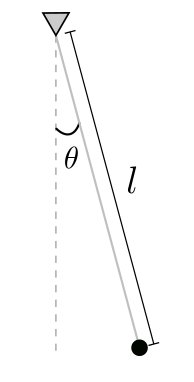
\includegraphics[scale=0.5]{figs/simplependulum.png}
%     \caption{The Simple Pendulum}
%     \label{simple}
% \end{figure}

% If a pendulum is set in motion so that is swings back and forth, its motion will be periodic. The time that it takes to make one complete oscillation is defined as the \textbf{time period} $T$ of the pendulum. Most of you will probably recognise the following formula for $T$: 

% \begin{equation}
%     T = 2 \pi \sqrt{\frac{l}{g}} 
%     \label{TimeP}
% \end{equation}

% where $l$ is the length of the pendulum from its fixed point, and $g$ is the acceleration due to gravity. Not so many of you, however, will realise that this is only true for \textbf{small displacements} around the equilibrium position. In general, when the pendulum is displaced from its equilibrium position, it experiences a restoring force $m g \sin\theta$. The differential equation describing its motion can be obtained from Newton's Second Law  $m\vb{a} = \vb{F}$.

% \begin{equation}
%     m l \dv[2]{\theta}{t} = - m g \sin\theta
% \end{equation}

% This is a difficult differential equation to solve. In the approximation that the angle $\theta$ is very small, we can replace $\sin\theta \approx \theta$, and we are left with the following differential equation:

% \begin{equation}
%     \dv[2]{\theta}{t} + \frac{g}{l} \theta = 0
% \end{equation}

% It is in this approximation that the simple pendulum is a \textbf{simple harmonic oscillator}, a very important model that you will not stop seeing the end of. In general, a quantity $Q$ is considered observe simple harmonic variation with respect to some parameter $t$ (not necessarily time) if it satisfies the following differential equation:

% \begin{equation*}
%     \dv[2]{Q}{t} + \omega_0^2 Q = 0
% \end{equation*}

% where $\omega_0$ is the time period of the oscillation, and is related to the time period of the oscillation through 

% \begin{equation*}
%     T = \frac{2\pi}{\omega_0}
% \end{equation*}

% Comparing, you should see that in our case, $$\omega_0 = \sqrt{\frac{g}{l}}$$ and $$T = 2\pi \sqrt{\frac{l}{g}}$$

% Thus, it should be clear that it is only when the amplitude is \textbf{small} that the time period follows this equation, since it is only then when you can approximate $\sin\theta$ with $\theta$.

% In this introductory experiment you will begin by verifying the above formula for the time period for small angles. You will then attempt to explore any variation of the time period with angle.